\section{Emerging Patterns}
\label{sec:patterns}

Despite the limited experience we hitherto gathered using \conesc, we
already observe quite distinctive design and programming patterns,
representing solutions to commonly occurring problems. % In general,
% however, they cannot be directly transformed into executable code
% without proper application-specific implementations.

% \conesc, as we mentioned before, makes the components of application more
% decoupled and reusable. To show that, we provide three possible patters --
% general solutions to a commonly occurring problems. 

\fakepar{Behavior control} Programmers often employ a single context
group to specify different \emph{behaviors} for the same high-level
functionality. One such example is the ``Base-station'' group in
Figure~\ref{fig:design}, which includes two different behaviors for
the functionality to report contact logs to the users. The
functionality itself is exported by one or more layered functions
defined in the group. The chosen behavior is then determined by
activating a single context within the group.

We found similar designs in other applications as well. In the
adaptive protocol stack, for example, the packet relay functionality
also matches a similar design. Depending on a node's mobility, the
chosen behavior is picked out of a pool of available protocols, whose
functionality are encapsulated in single contexts. These are in turn
included in a single context group, which exports a layered function
where the application layers transparently accesses whatever protocol
is in operation at a given time.

% Whenever the application should perform some specific
% actions repeatedly, according to the environmental conditions, the developer
% should use \emph{Behavior Control Pattern}. The example is in our scenario, when
% the application adapts to the reach-ability of the base-station.

Figure~\ref{fig:control} shows an abstract view of such commonly
recurring pattern. In addition to the context group exporting the
adaptive functionality and the single contexts therein, programmers
also define an additional ``controller'' component, which activates
the single contexts within the group depending on the
situation. Figure~\ref{fig:bscm} shows one such example for the
wildlife monitoring application. Similar designs apply to the
smart-home controller and the adaptive protocol stack as well.

\begin{figure}
\begin{center}
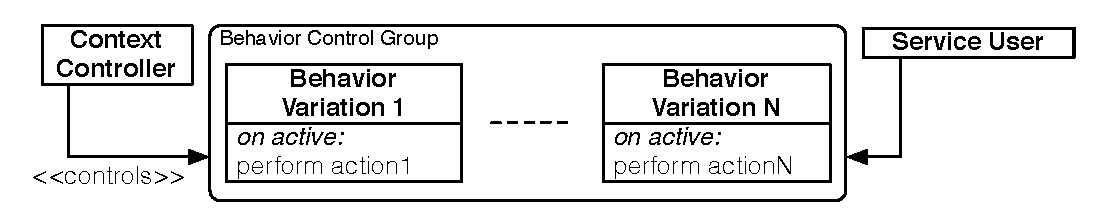
\includegraphics[scale=.5]{imgs/beh_var}
\vspace{-1mm}
\caption{Behavioral control pattern.}
  \label{fig:control}
\vspace{-8mm}
\end{center}
\end{figure}

% Context group in that case includes the functionality, which needs to adapt.
% Each context implies an implementation of a corresponding functionality. 

% To make the pattern complete, we also use a separate control module,
% which is responsible only for the activating suitable context in the
% given context group. Since this pattern controls the behavior of the
% device, it is mostly applicable in the system level.

% Behavior Control Pattern can also be applied on Smart-home system, when system
% needs to send data to the Fire, or Police, or both, depending on the type of
% emergency. The Adaptive protocol can also use this pattern to switch between
% CTP- or Gossip-based protocols depending on the network topology.

\fakepar{Content provider} Different from the behavior control
pattern, which provides non-trivial context-dependent processing, we
observe cases where context-dependent \emph{data} is offered to other
functionality with little to no processing involved. In the wildlife
monitoring application, for example, the ``Health conditions'' group
in Figure~\ref{fig:design} provides differently formatted beacons to
the radio driver for broadcast transmissions. Layered functions are,
in this case, defined for the group merely to retrieve the
context-dependent data.

In this case as well, we notice the same pattern in other
applications. In the smart-home controller, for example, a context
group is defined to manage the user preferences depending on day vs.\
night. These data are simply retrieved differently from a common data
storage by two different contexts modeling day or night
situations. Whatever user preference is to be considered at a given
point is then handed over to the control loop in charge of setting the
functioning of the climate systems.

\begin{figure}
\begin{center}
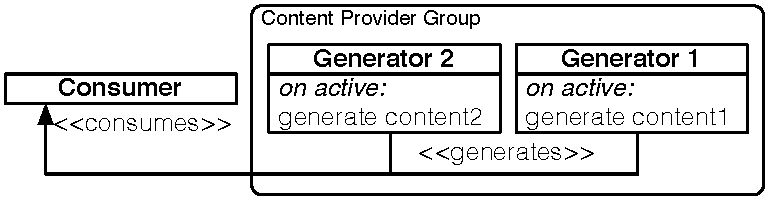
\includegraphics[scale=.5]{imgs/content_provider}
\vspace{-1mm}
\caption{Content provider pattern.}
  \label{fig:provider}
\vspace{-8mm}
\end{center}
\end{figure}

As shwn in Figure~\ref{fig:provider}, this pattern's structure differs
from that of behavior control in that the role of the ``controller''
component is often fairly trivial (and hence omitted in the
picture). In the smart-home controller, for example, the controller
component is simply based on the time of the day. On the other hand,
the component consuming the context-dependent data plays a key
role. Indeed, while functionality structured according to behavior
control can be considered stand-alone, the context provider needs to
be tailored to the data consumer.

\fakepar{Trigger} We also recognize designs where single contexts are
used only to trigger specific operations when entering/exiting a
context, but no significant context-dependent functionality or data is
offered as the context remains active. One example in the wildlife
monitoring application is the ``Battery'' group in
Figure~\ref{fig:design}. The included contexts are used to
enable/disable the GPS sensor depending on battery levels, but no
other functionality is provided to other components. In this
case, layered functions are often not defined, in
that the predefined \code{activated} and \code{deactivated} events
within the single contexts suffice.

In the smart-home controller, for example, we notice a similar pattern
in the context group regulating light dimming. Depending on
perceived light levels in a room, either context ``Too bright'' or
``Too dark'' is activated, and lights are tuned accordingly when
entering either context. This processing is entirely implemented
within the corresponding \code{activated} event handlers. 

In more general terms, a ``controller'' component is present in this
case as well to drive the context transitions in the group, as shown
in Figure~\ref{fig:trigger}. However, unlike the other patterns, there
is no other component that either uses context-dependent functionality
or consumes context-dependent data.

\begin{figure}
\begin{center}
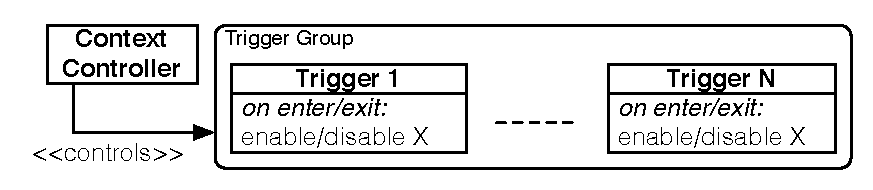
\includegraphics[scale=.5]{imgs/con_act}
\vspace{-1mm}
\caption{Trigger pattern.}
  \label{fig:trigger}
\vspace{-8mm}
\end{center}
\end{figure}

%%% Local Variables: 
%%% mode: latex
%%% TeX-master: "paper"
%%% End: 
